\section{Метод №4}\label{meth4}

\subsection{Идея}\label{math4:idea}

\begin{itemize}
	\item[1)] Проводим прямые через точки множеств в направлениях проектирования и получаем множество скрещивающихся прямых.
	\item[2)] Рассматривая искомую прямую как вектор, приложенный к точке, составляем функционал суммы квадратов расстояний от прямой до множества скрещивающихся прямых и минимизируем его: получаем нелинейную систему, которую решаем доступными способами.
	
\end{itemize}

\vspace{0.5cm}
\begin{center}
	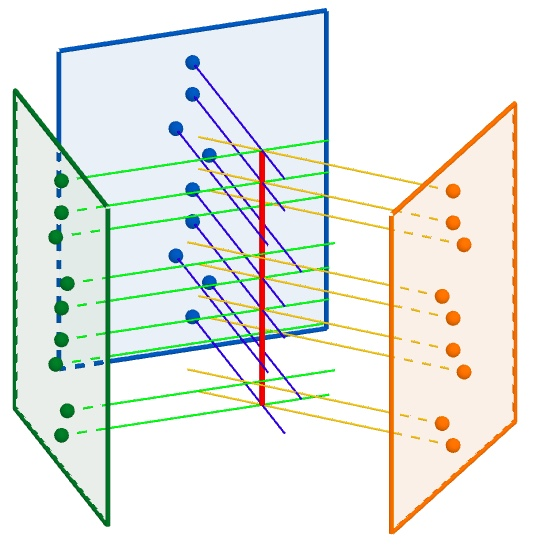
\includegraphics[scale=0.7]{131}

	Рис. 2.7: Построение скрещивающихся прямых через точки множеств.
\end{center}

\newpage
\subsection{Решение}\label{math4:solution}

Алгоритм аналогичен методу 3 \ref{math3:solution}, т.е. имеем задачу по нахождению минимального значения выражения
$$\underset{j=1}{\overset{3}{\sum}} \underset{i=1}{\overset{n_1, n_2, n_3}{\sum}}
\frac{\left(\triangle_{ij}^x (n r_3^j - p r_2^j) - \triangle_{ij}^y (m r_3^j - p r_1^j) + \triangle_{ij}^z (m r_2^j - n r_1^j)\right)^2}{(n r_3^j - p r_2^j)^2 + (p r_1^j - m r_3^j)^2 + (m r_2^j - n r_1^j)^2}$$
по шести параметрам: $m,n,p$ (компоненты вектора искомой прямой) и $x_0, y_0, z_0$ (координаты точки, лежащей на искомой прямой).

\subsection{Погрешность и примеры работы программ}\label{math4:error}

ждет заполнения

